%!TEX root = ../report.tex

\begin{document}
    \justifying
    \chapter{Related Work}
    \label{related_work}

    This chapter provides an overview of the most common methods and architectures proposed to solve the task of object detection. It continues to furnish an outline about some \acrlong{ood} (\acrshort{ood}) detection methods applied to solve classification tasks in computer vision.

    \section{Object Detection}
    \label{OD_methods}
    In general, object detection is defined as \textit{"determining whether are not the instances of objects present in the image and localizing them"}. The location of the objects is coarsely encoded as a bounding box \textit{an axis-aligned rectangle tightly bounding the object of interest}. The task of solving object detection depends on each class of objects having features that are very distinctive from one class to another. These features are utilized further to find the interesting regions in the image consisting of the objects. Object detection methods are historically classified into two main categories: \textit{traditional machine learning-based methods}, which uses carefully hand-crafted features and classify them using machine learning methods, and \textit{deep learning-based methods}, which uses Convolutional Neural Networks (CNNs) to extract features by learning from experience. In this work, we majorly concentrated on deep learning-based object detection in a 2-Dimensional (2D) setting.
    
    In deep learning-based 2D object detection, models are divided into region-based (Two Stage) and unified (Single Stage) models.
    
    \subsection{Region based (Two Stage) frameworks}
    The two-stage object detection model takes an RGB image as input. The model initially extracts category-independent region proposals using selective search or region proposal network. A classifier then process generated proposals to extract bounding box coordinates and objects class. The seminal works in two-stage object detectors belong to Regions with Convolutional Neural Networks (RCNN) family proposed \cite{Girshick2014}. 
    
    RCNN proposed by \citet{Girshick2014} integrates AlexNet \cite{AlexNet2012} and selective search \cite{uijlings2013} to detect the objects in an image. Class independent region proposals that might contain any object of interest are proposed using selective search. Image is cropped and warped based into similar sizes based on the region proposals and are used to train a CNN model which is pre-trained for classification tasks on another dataset like ImageNet \cite{imagenet}. Class-specific Support Vector Machines (SVMs) are trained using the fixed-length features extracted using CNN. This SVM replaces the softmax layer present in the CNN. Class-specific bounding box regressor extracts bounding box values from the features extracted by the CNN. Though RCNN was able to outperform the existing models in terms of detection quality it suffered from many drawbacks. More notably, training an RCNN model is slow and hard to optimize due to the need for training various sub-models independently. Also, the amount of computational and memory requirements are high due to the requirement for features needed to train the SVM are to be stored. Also, the inference time is high due to the extraction of per object proposal for every test image.
    
    % \begin{figure*}[!htbp]
    %     \centering
    %     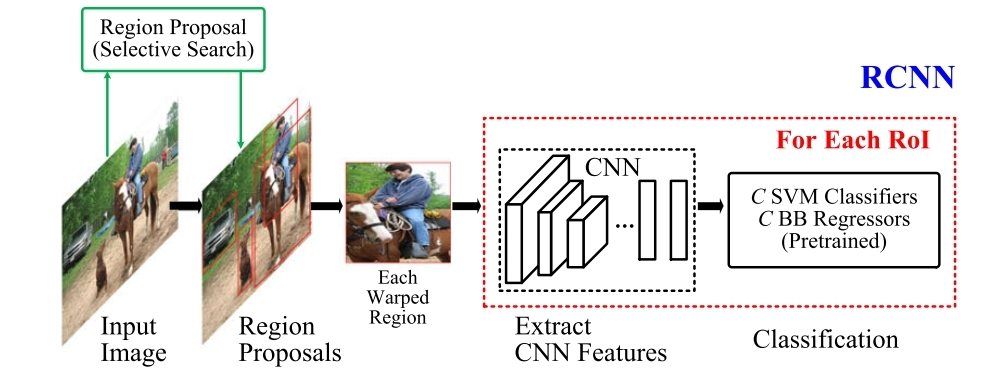
\includegraphics[scale=0.4]{images/frameworks/RCNN.jpg}
    %     \caption{RCNN framework proposed}
    %     \label{fig:RCNN}
    % \end{figure*}
    
    To address the disadvantages in the RCNN model, another method Fast RCNN is proposed by \citet{Girshick2015}. In this model whole image is processed by CNN to generate object proposals. A feature vector is extracted from each of the proposals generated using a Region Of Interest (ROI) pooling layer this essentially acts as a learned warping function at the feature level. The extracted features are passed through a stack of Fully Connected (FC) layers and divided into two different heads, one with a softmax layer which acts as a classifier and another head extracts class-specific bounding box offsets which are used for the further refinement of object proposals. The most important step that the Fast RCNN model introduced is the ability to train the object detection network in an end-to-end manner. This model resulted in reducing the training time by three-fold while the inference speeds are improved by 10 times. Another most important optimization is done in memory required with the removal of feature caching required for training the RCNN model. Though Faster RCNN sped up the training and inference speeds by multiple folds, it still depended on the externally generated region proposals which are exposed as a bottleneck for real-time applications.
    
    % \begin{figure*}[!htbp]
    %     \centering
    %     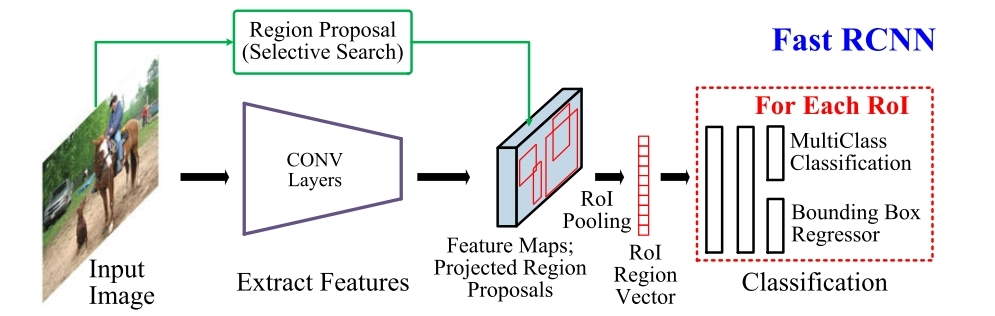
\includegraphics[scale=0.4]{images/frameworks/Fast-RCNN.jpg}
    %     \caption{RCNN framework proposed}
    %     \label{fig:F-RCNN}
    % \end{figure*}
    
    Faster RCNN is a third-generation RCNN model proposed by \citet{Ren2017} which uses the CNNs ability to localize objects using convolutional layers. Hence, Faster RCNN used an efficient Region Proposal Network (RPN) for generating region proposals. RPN is shared for region proposal generation and also for performing a classification task. RPN initially produces \textit{k} boxes referred to as \textit{anchor boxes}, which are of different scales and aspect ratios at each Convolutional feature map location. These anchor boxes are generated independent of the image content but the features generated by the convolution layers from these anchor boxes are image content dependent. Each feature extracted from an anchor box is fed to a stack of FC layers which is further branched into a classification network and a box regression network.
    
    % \begin{figure*}[!htbp]
    %     \centering
    %     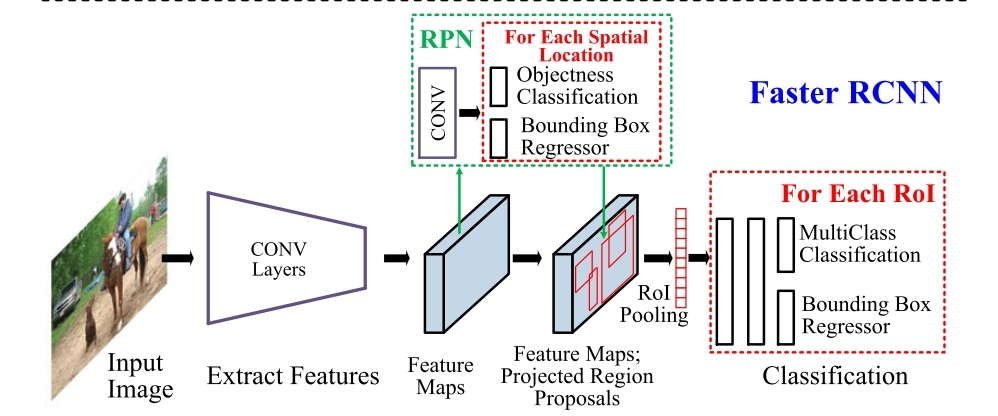
\includegraphics[scale=0.4]{images/frameworks/Faster-RCNN.jpg}
    %     \caption{Faster RCNN framework proposed}
    %     \label{fig:Fr-RCNN}
    % \end{figure*}
    
    \subsection{Unified (Single Stage) frameworks}
    The region-based frameworks are computationally expensive in devices with less storage or computational ability. This drawback in region-based networks had accelerated the research in unified frameworks. The unified framework predicts the object class and regresses the bounding box offsets from the input image in a single forward-pass. These models avoid the usage of region proposal generation or feature post-processing.
    
    The pioneering work in unified frameworks is You Only Look Once (YOLO) proposed by \citet{Redmon2016}, which divides an image into a 7 x 7 grid and performs classification and localization on each cell in parallel. It is observed that framing the object detection problem as a regression problem resulted in reduced processing time.  It outperformed the Deformable Part Model (DPM) proposed by \citet{DPM} and R-CNN \citet{Girshick2014}. This method struggle from not being able to detect objects of smaller sizes. There were revisions done to the initial YOLO models proposed by the same authors and proposed YOLOv2 and YOLOv3, though there are improvements in detection accuracy it is not considerable. A considerable update is done in YOLOv4 proposed \citet{Bochkovskiy2020} in which authors used different strategies in data augmentation (Mosaic, CutMix, Label smoothing), loss functions for bounding box (IoU loss, GIoU loss, DIoU loss, CIoU loss), and activation functions (leaky-ReLU, Swish, Mish). The model trained using the above advancements led to an increase in the Average-Precision (AP) values from 38.0\% to 42.4\%.
    
    % \begin{figure*}[!htbp]
    %     \centering
    %     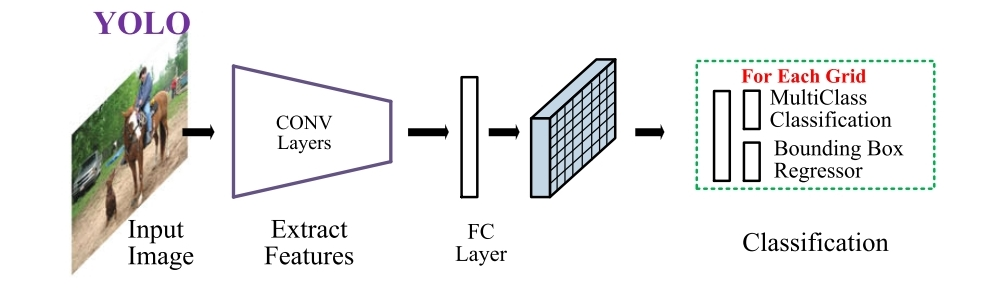
\includegraphics[scale=0.4]{images/frameworks/YOLO.jpg}
    %     \caption{YOLO framework proposed}
    %     \label{fig:Fr-RCNN}
    % \end{figure*}

    Single Shot Multi-box Detector \citet{Liu2016SSDSS} is another single-stage object detector model in which object detection is done at several different layers of CNN instead of only doing it from the last layer. This technique allows us to detect objects of different sizes and also improved the accuracy predominantly. The current State-Of-The-Art (SOTA) object detector is EfficientDet proposed by \citet{Tan2020}. The authors proposed Bi-directional Feature Pyramid Network (Bi-FPN) in which a modified feature pyramid network proposed by \citet{Liu2018} is used as a base network and is modified by varying the connections in Bi-FPN to modify the intermediate features to consider thereby increasing the accuracy along with several parameters that the model constitute. The authors also proposed a compound scaling method, which performs the up-scaling of resolution for regression of bounding box and objects classification. Eight different EfficientDet networks are starting from D0 to D7, which is controlled with compound scaling coefficient $\phi$.
    
    % \begin{figure*}[!htbp]
    %     \centering
    %     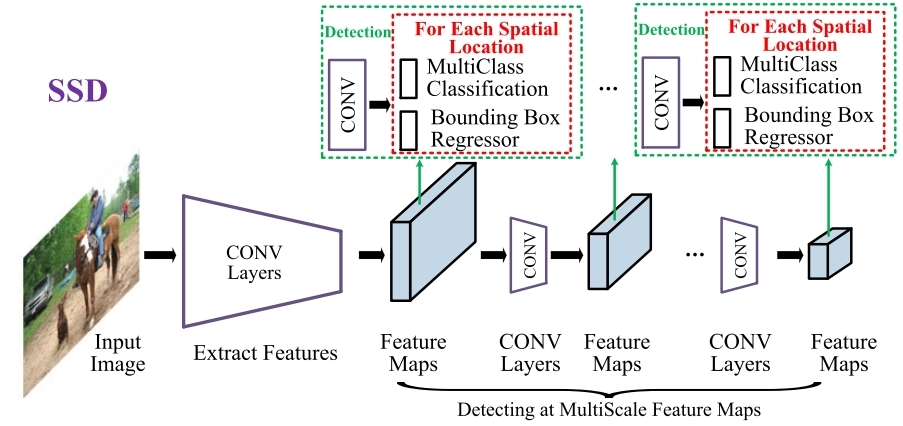
\includegraphics[width=15cm, height=5cm]{images/frameworks/SSD.jpg}
    %     \caption{SSD framework proposed}
    %     \label{fig:Fr-RCNN}
    % \end{figure*}
    
    \subsection{Object-Detection Metrics}
    In this section, we present various metrics that are used to measure the performance of the object detectors.
    \subsubsection{Intersection over Union}
    Intersection over Union (IoU) is an evaluation metric that is employed to measure the detection accuracy of an object detector. To apply this metric we need ground-truth encoding of the bounding box and the encoding label of the bounding box. IoU is computed using Equation \ref{IoU}, as the area of intersection between the predicted bounding box and ground-truth bounding box divided by the area from the union of the boxes. An IoU value of unity implies the two bounding boxes are identical.
    
    \begin{equation}
        IoU = \frac{\textit{Area of intersection of predicted and ground truth boxes}}{\textit{Area of union of predicted and ground truth boxes}}
        \label{IoU}
    \end{equation}
    
    \subsubsection{Precision and Recall}
    Precision refers to the percentage of your results that are relevant and Recall refers to the percentage of total relevant results correctly classified by the model. An object detector is performing well if its precision is high with an increase in recall value. Precision and Recall are calculated using True Positive, False Positive, and False Negative rates.
    
    \begin{equation}
    Precision = \frac{TP}{\textit{TP + FP}}
    \end{equation}
    
    \begin{equation}
    Recall = \frac{TP}{\textit{TP + FN}}
    \end{equation}
    
    \subsubsection{Average Precision}
    Average precision summarizes the precision value for 11 equally spaced recall values i,e. [0, 0.1, 0.2,.....,1]. The precision for each recall level is calculated as the maximum precision value measured where the corresponding recall is greater than or equal to the corresponding recall value.
    
        \begin{equation}
            \mathrm{AP}=\frac{1}{11} \sum_{r \in\{0,0.1, \ldots, 1\}} p_{\text {interp }}(r)
        \end{equation}
        
        \begin{equation}
            p_{\text {interp }}(r)=\max _{\hat{r}: \vec{r} \geq r} p(\tilde{r})
        \end{equation}
    
    \subsubsection{Mean Average Precision}
    The metric \acrlong{map} (\acrshort{map}) is introduced to evaluate the performance of object detectors in which there is more than one foreground class. \acrshort{map} is the mean of the per-class \acrshort{ap} scores.

    \section{Out-Of-Distribution Detection}
    \label{OOD_Detection}
    As mentioned in Section \ref{OD_methods} the majority of well-performing object detection methods are learning-based. But, the majority of the existing learning-based models are evaluated on the assumption that the test data are drawn from independent and identical distribution ($i.i.d$) also known as In-Distribution (ID). However, in a real-world deployment of these models might need to infer samples that can be Out-Of-Distribution (OOD). The distribution shift between OOD and ID stems from either \textit{semantic shift} (samples from different class)  or \textit{covariate shift} (samples from a different domain). 
    
    Class setting in OOD detection is visualized in Figure \ref{fig:OOD_classes} and consists of following problems
    \begin{itemize}
        \item \textbf{Sensory anomaly detection}: the samples with covariate shift from train images are considered OOD. No semantic shift can be observed. 
        \item \textbf{Semantic anomaly detection or one-class novelty detection}: the sample images with semantic shift will be considered as OOD. No covariate shift is observed. 
        \item \textbf{Multi-Class novel detection}: ID images consists of multiple classes to detect. while, samples with semantic shift will be considered OOD. No covariate shift is observed in the test samples. 
        \item \textbf{Open-set recognition}: is a similar setting as multi-class novelty detection but includes classification of classes in in-distribution samples. 
        \item \textbf{Out of Distribution detection}:  \acrshort{ood} detection is a super-set which includes semantic anomaly detection, one-class novelty detection, multi-class novelty detection and open-set recognition that aims at detecting samples with semantic-shift without deteriorating its performance on ID dataset.
    \end{itemize}
    
    \begin{figure*}[!htbp]
        \centering
        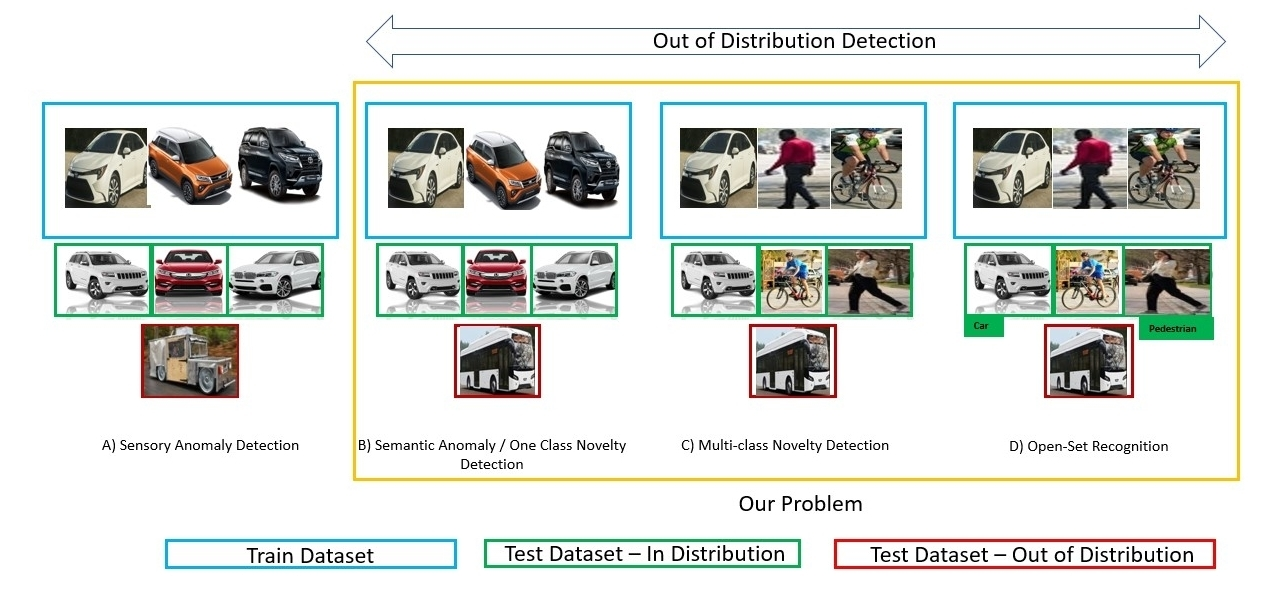
\includegraphics[scale=0.35]{images/OOD_vs_Non-OOD.jpg}
        \caption[\acrlong{ood} detection problem setting]{Class differentiation in generalized OOD detection framework}
        \label{fig:OOD_classes}
    \end{figure*}
    
    Out-of-distribution detection methods classify the inputs that are sampled from another distribution from the inputs used for training the inference model. These methods can be classified into four different groups: Metric, Inconsistency, Generative, and Uncertainty based approaches.
    \subsection{Metric based methods}
    Metric methods determine if the input is OOD based on the behavior of the current input following the behavior of the samples inside the generalization area of the DNN under investigation. 
    
    One of the works done is by \citet{Devries} in which a classification model is modified to output an additional value $c$ along with a softmax score. The training pipeline is modified to include a two-folded loss while penalizing a misclassification using cross-entropy loss along with a penalty for lower confidence score $c$. Another method proposed by \citet{Oberdiek2018} in which intermediate values like layerwise norm, minimum and maximum value of the layer-wise gradient of the weights with respect to the loss function of the predicted class are fed to a logistic regressor along with entropy of the output class. The logistic regressor produces a score value which helps in deciding whether an input is OOD. 
    
    \citet{Hendrycks2018} also adapts the training procedure of the classification model. The authors extract a carefully curated dataset that contains samples outside the generalization area and assign a uniform distribution of values over all the classes as the labels and are used while training along with the original training dataset. An input leading to output with higher entropy is judged to be an OOD sample. Another work proposed by \citet{Lee2018} computes Mahalanobis distance between activation space of the DNN layers to the closest class-conditional Gaussian distribution. All the layerwise distances are fed to a logistic regression network which outputs a score value to decide whether the input is an OOD input.
    \subsection{Inconsistency based methods}
    The basic idea behind inconsistency-based methods is to induce a minimal change to the sample from the in-distribution dataset. During inference, both the image and the modified image are processed and the distance between the outputs is used to classify the in-distribution sample and OOD sample.
    
    ODIN proposed by \citet{liang2017enhancing} in which the OOD detection is done by scaling the logit layers before the softmax output by a constant value called temperature, as well as perturbs the image input by a small amount. A sample is expected to be in distribution if the output value of the modified image for the original predicted class is high. These methods had resulted in the best performing model for detecting OOD data points. 
    \subsection{Generative methods}
    Generative methods are similar to inconsistency-based methods except in the way perturbation to the input images is performed. The perturbation is made to shift the image more towards the training distribution and is made using a generative network trained on the in-distribution training dataset. During inference, both the original and the generated image are processed, and the higher the distance between both outputs the confident we are that the input sample is OOD.
    
    One method proposed using this philosophy is proposed by \citet{Hendrycks2017} in which an encoder is employed on top of the penultimate layer of the original DNN, which helps in reconstructing the image. The difference between the original image and the generated image along with the output of the final layer and the penultimate layer to an abnormality module which regresses the confidence score that can be used to differentiate OOD input from an in-distribution input. Another such work is proposed by \citet{Ren2019} in which the authors used likelihood ratio value. if the likelihood ratio determined between the output of the model trained on the original images and the one on the perturbed images is low, the input image is expected to be OOD. The authors had trained two generative PixelCNN models by \citet{VanDenOord2016}, one on the original dataset and another on the slightly perturbed images from the training dataset. From the observation, they concluded that the model trained on original images is sensitive to the true class contents compared to the model trained on perturbed data. Hence, a low likelihood ratio value points to an OOD input.  
    
    \subsection{Uncertainty based methods}
    An uncertainty measure could be directly applied to reject OOD samples as we would expect the uncertainty to be high on such inputs. There are multiple uncertainty types coined in various researches proposed by \citet{MacKay1992, MacKayThesis1992, Radford1996}. The uncertainty extracted using Bayesian approaches is called epistemic uncertainty which measures the uncertainty in estimating the model parameters given the training data. In other words, epistemic uncertainty measures how well the model is matched to the data in terms of model structure and parameters. The other type of uncertainty is aleatoric uncertainty, which is irreducible uncertainty that arises from the natural complexity of the data, e.g. from class overlap or label noise. Some works presented by \citet{JimThesis1992, Lakshminarayanan2017, VanAmersfoort2020} had presented an argument that OOD data is implicitly modeled by epistemic uncertainty.
    
    Exploiting this idea, \citet{Lakshminarayanan2017} proposed the usage of an ensemble of multiple models to extract epistemic uncertainty which can be used to judge whether an input is from in-distribution. Similarly, \citet{Malinin2018} proposed prior networks for uncertainty estimation and dis-entangle the predictive uncertainty into three contributing factors model uncertainty, data uncertainty, and distributional uncertainty. The authors used distributional uncertainty, which arises when input is sampled from a distribution that is very different from the training distribution. 
    
    \section{\acrlong{ood} methods - Deep Dive}
    In this section, we provide background information about various classical \acrshort{ood} detection methods used in this thesis. This section differs from Section \ref{OOD_Detection} in providing deep-dive information in explaining why the \acrshort{ood} detector works.
    \subsection{Max Softmax Probability}
    The work proposed by \citet{hendrycks17baseline} proposed a metric to separate the In-Distribution (ID) sample from the Out-Of-Distribution (OOD) sample which uses maximum softmax confidence score from the softmax layer of the network. The authors' reasoning in using the softmax score as a metric is though the network yields over-confident scores for the OOD sample. But these confidence values are often lower than the probability with which ID samples are classified.
    
    Following the above reasoning, the authors used the Equation \ref{softmax_score} to obtain a maximum value of softmax scores which can be used as a novelty score to classify an ID and OOD sample.
    \begin{equation}
    \setlength{\jot}{10pt}
        s\left(\mathbf{x}^{*}\right)=\max _{c} P\left(y_{c} \mid \mathbf{x}^{*} ; \mathcal{D}\right)
        \label{softmax_score}
    \end{equation}
    
    In Equation \ref{softmax_score}, $\mathbf{x}^{*}$ is the sample that belongs either to an ID class or to an OOD class, $y_{c}$ is the class label, and $P\left(y_{c} \mid \mathbf{x}^{*} ; \mathcal{D}\right)$ is an estimation of class specific probabilities from a Neural Network (NN) trained on dataset $\mathcal{D}$
    
    \subsection{ODIN}
    \label{odin_explained}
    ODIN is a post-hoc method proposed by \citet{Liang2017}, it is mentioned as a post-hoc method as there is no modification of training is needed to separate ID and OOD samples. This method out-performed Max Softmax Probability by using the scaling of logit layers before the softmax layer of a neural network by a Temperature value $\mathbf{T}$ along with a small gradient-based perturbation added to the input image. 
    
    In this work, the author used images from CIFAR-10 and CIFAR-100 as ID samples and images from TinyImageNet, LSUN, and artificially generated datasets made up of Uniform and Gaussian noise. 
    
    \subsubsection{Temperature Scaling}
    In previous works, Temperature scaling is a method used in distilling the knowledge in neural networks by \citet{Hinton2015DistillingTK} and for calibrating the confidence scores in classification tasks by \cite{GuoCalibration2017}. ODIN proposed by \citet{Liang2017} observed from various experimentation that temperature scaling also can be used to separate ID and OOD samples.
    
    For a neural network $\mathbf{f}$ that is trained on a dataset for multi-class classification. For an input $\mathbf{x}$, we calculate softmax scores using the Equation \ref{ODIN_Softmaxscore}. The class with maximum softmax probability $S_{\hat{y}}(\boldsymbol{x} ; T)=\max _{i} S_{i}(\boldsymbol{x} ; T)$ is used as class output.
    
    \begin{equation}
        S_{i}(\boldsymbol{x} ; T)=\frac{\exp \left(f_{i}(\boldsymbol{x}) / T\right)}{\sum_{j=1}^{N} \exp \left(f_{j}(\boldsymbol{x}) / T\right)}
        \label{ODIN_Softmaxscore}
    \end{equation}
    
    To show the effectiveness of Temperature we perform Taylor expansion of the softmax function presented in Equation \ref{ODIN_Softmaxscore},
    
    \begin{equation}
        \begin{aligned}
            S_{\dot{y}}(\boldsymbol{x} ; T) &=\frac{\exp \left(f_{\hat{y}}(\boldsymbol{x}) / T\right)}{\sum_{i=1}^{N} \exp \left(f_{i}(\boldsymbol{x}) / T\right)} \\
            &=\frac{1}{\sum_{i=1}^{N} \exp \left(\frac{f_{i}(\boldsymbol{x})-f_{y}(\boldsymbol{x})}{T}\right)} \\
            & \text {performing Taylor expansion and neglecting the terms from $3^{rd}$ order and above, we get} \\
            &=\frac{1}{\sum_{i=1}^{N}\left[1+\frac{f_{i}(\boldsymbol{x})-f_{\dot{j}}(\boldsymbol{x})}{T}+\frac{1}{2 !} \frac{\left(f_{i}(\boldsymbol{x})-f_{\hat{j}}(\boldsymbol{x})\right)^{2}}{T^{2}}+o\left(\frac{1}{T^{2}}\right)\right]} \\
            & \approx \frac{1}{N-\frac{1}{T} \sum_{i=1}^{N}\left[f_{\hat{y}}(\boldsymbol{x})-f_{i}(\boldsymbol{x})\right]+\frac{1}{2 T^{2}} \sum_{i=1}^{N}\left[f_{i}(\boldsymbol{x})-f_{\hat{y}}(\boldsymbol{x})\right]^{2}}
        \end{aligned}
        \label{Temperatue_effect}
    \end{equation}
    
    Let us represent, $f_{\tilde{y}}(x)-f_{i}(x)$ as $\Delta_{i}$ and set of $\Delta_{i}$ over all classes be $\Delta$. Hence, $\Delta=\left\{\Delta_{i}\right\}_{i \neq \hat{y}}$ and $\bar{\Delta}$ denote the mean of the set $\Delta$. The first term after summation in the denominator is represented as $U_{1}$
    
    \begin{equation}
        U_{1} = \bar{\Delta}=\frac{1}{N-1} \sum_{i \neq \hat{y}} \Delta_{i}=\frac{1}{N-1} \sum_{i \neq \hat{y}}\left[f_{\hat{y}}-f_{i}\right]
        \label{u1}
    \end{equation}
    
    The second term after summation in the denominator can be represented as $U_{2}$ and further expanded to understand the effect of Temperature Scaling:
    
    \begin{equation}
        \setlength{\jot}{10pt}
        \begin{aligned}
        U_{2} & =\frac{1}{N-1} \sum_{i \neq \hat{y}} \Delta_{i}^{2} & \text { by } \Delta_{i}=f_{\dot{y}}-f_{i} \\[7.5pt]
        & =\frac{1}{N-1} \sum_{i \neq \hat{y}}\left(\Delta_{i}-\bar{\Delta}+\bar{\Delta}\right)^{2} & \\[7.5pt]
        & =\frac{1}{N-1} \sum_{i \neq \bar{y}}\left[\left(\Delta_{i}-\bar{\Delta}\right)^{2}-2\left(\Delta_{i}-\bar{\Delta}\right) \bar{\Delta}+\bar{\Delta}^{2}\right] & \\[7.5pt]
        & =\underbrace{\frac{1}{N-1} \sum_{i \neq \bar{y}}\left[\Delta_{i}-\bar{\Delta}\right]^{2}}_{\operatorname{Variance}^{2}(\Delta)}-\underbrace{\frac{2 \bar{\Delta}}{N-1} \sum_{i \neq j}\left(\Delta_{i}-\bar{\Delta}\right)}_{=0}+\underbrace{\bar{\Delta}^{2}}_{\operatorname{Mean}^{2}(\Delta)}
        \end{aligned}
        \label{u2}
    \end{equation}
    
    From Equation \ref{u1}, we can observe that $U_{1}$ measures How much the dominant value of the output of the neural network deviates from the remaining outputs, and from Equation \ref{u2} measures the variance of all the remaining outputs.
    
    Referring back to Equation \ref{Temperatue_effect}
    \begin{equation}
        \begin{gathered}
            S_{y}(x ; T)=\frac{1}{N-\frac{1}{T} \sum_{i-1}^{N}\left[f_{i}(x)-f_{i}(x)\right]+\frac{1}{2 T^{2}} \sum_{i-1}^{N}\left[f_{i}(x)-f_{\hat{y}}(x)\right]^{2}} \\[7.5pt]
            \mathrm{U}_{1}=\frac{1}{N-1} \sum_{i \neq \hat{y}}\left[f_{\hat{y}}(x)-f_{i}(x)\right] \\[7.5pt]
            \mathrm{U}_{2}=\frac{1}{N-1} \sum_{i \neq \hat{y}}\left[f_{\hat{y}}(x)-f_{i}(x)\right]^{2} \\[7.5pt]
            S_{y}(x ; T)=\frac{1}{N\left(1-\frac{1}{(N-1) T} \sum_{i \neq \hat{y}}\left[f_{\hat{y}}(x)-f_{i}(x)\right]+\frac{1}{2(N-1) T^{2}} \sum_{i+\hat{y}}\left[f_{\hat{y}}(x)-f_{i}(x)\right]^{2}\right)} \\[7.5pt]
            =\frac{1}{N\left(1-\frac{1}{T}\left(U_{1}-\frac{U_{2}}{2 T}\right)\right)}
        \end{gathered}
        \label{Softmax_modifications}
    \end{equation}
        
    From the Equation \ref{Softmax_modifications}, we can conclude that $S \propto\left(U_{1}-U_{2} / 2 T\right) / T$. The component $U_{1}$ results in producing larger softmax scores for in-distribution images than out-of-distribution images. But $U_{2}$ has inverse-proportion effect on softmax scores $S \propto-U_{2}$. 
    Choosing a large temperature reduces the negative effects of $U_{2} / 2 T$ resulting in in- and out-of-distribution samples being more distinguishable.
    
    \subsubsection{Input Preprocessing}
    The authors also proposed to perform input pre-processing by subtracting a small perturbation noise to the input image. This approach is inspired by the work done by \citet{Goodfellow2015} in which a small perturbation is added to make the softmax scores less effective for classification purposes thereby forcing the neural network to make an incorrect prediction. 
    
    \begin{equation}
        \tilde{\boldsymbol{x}}=\boldsymbol{x}-\operatorname{esign}\left(-\nabla_{\boldsymbol{x}} \log S_{\hat{y}}(\boldsymbol{x} ; T)\right)
        \label{perturbation}
    \end{equation}
    
    \begin{equation}
        \log S_{\tilde{y}}(\tilde{\boldsymbol{x}} ; T)=\log S_{\dot{y}}(\boldsymbol{x} ; T)+\varepsilon\left\|\nabla_{\boldsymbol{x}} \log S_{\dot{y}}(\boldsymbol{x} ; T)\right\|_{1}+o(\varepsilon)
        \label{log_softmax}
    \end{equation}
    
    where $\epsilon$ is the perturbation magnitude and $S_{\hat{y}}(\boldsymbol{x} ; T)$ is the maximum temperature-scaled softmax scores produced by the network fed with an image $\boldsymbol{x}$. The authors had modified the input increasing softmax scores. This effect can be seen more in case in-distribution samples than out-of-distribution samples.
    
    The behavior of softmax score in case of input perturbation can be understood by analyzing the log-softmax function as shown in Equation \ref{log_softmax} with the input as perturbed image $\tilde{x}$. From extensive experimentation, the authors observed that the in-distribution samples tend to have a larger norm of gradients in comparison to out-of-distribution samples. In case of equal softmax values for in and out of distribution samples, But magnitude of gradients $L_{1}$ norm calculated using $|\nabla_{\boldsymbol{x}} \log S_{\dot{y}}(\boldsymbol{x} ; T) \|_{1} $ is high for in-distribution sample. 
    
    \subsection{Mahalanobis distance-based OOD Detector}
    \label{MD_ood}
    \citet{Lee2018} proposed Mahalanobis distance-based out-of-distribution detector which assumes that the intermediate layer features of pre-trained models following class-conditional Gaussian distributions with tied covariances for all class distributions, and the classification confidence score for a new input $\mathbf{x}$ is defined as the Mahalanobis distance from the closest class conditional distribution. Mahalanobis distance is calculated using the Equation 
     
    \begin{equation}
        \begin{gathered}
            M(x)=\max _{c}-\left(f(x)-\hat{\mu}_{c}\right)^{T} \hat{\Sigma}^{-1}\left(f(x)-\hat{\mu}_{c}\right), where. \\
            & \hat{\mu}_{c}=\frac{1}{N_{c}} \sum_{i: y_{c}=c} f\left(x_{i}\right) \\
            & \hat{\Sigma}=\frac{1}{N} \sum_{c} \sum_{i: y_{c}=c}\left(f\left(x_{i}\right)-\hat{\mu}_{c}\right)\left(f\left(x_{i}\right)-\hat{\mu}_{c}\right)^{T} \\
        \end{gathered}
        \label{Mahalanobis_dist}
    \end{equation}
    
    The authors assume that the class-priors follow categorical distributions $P(t=c)=\beta_{c} / \sum_{c^{\prime}} \beta_{c^{\prime}}$ and class-conditional distributions can be modelled as Gaussian distributions with tied covariance $\mathcal{N}\left(\mathbf{x} \mid \mu_{c}, \Sigma\right)$. 
    
    The Posterior can be defined as follows using Bayes theorem
    
    $$P(y=c \mid x)=\frac{P(x \mid y=c) P(x)}{P(x)}$$
    
    As already mentioned above that likelihood is a Gaussian distribution
    
    $$P(x \mid y=c)=\frac{1}{\sqrt{2 \pi \Sigma}} e \frac{-\left(x-\mu_{c}\right)^{T} \Sigma^{-1}\left(x-\mu_{c}\right)}{2}$$
    
    $$ P(y=c \mid x)=\frac{\frac{1}{\sqrt{2 \pi \Sigma}} e \frac{-\left(x-\mu_{c}\right)^{\top} \Sigma^{-1}\left(x-\mu_{c}\right)}{2}\left(\beta_{c}\right)}{\sum_{c^{\prime}} \frac{1}{\sqrt{2 \pi \Sigma}} e \frac{-\left(x-\mu_{c}^{\prime}\right)^{\top} \Sigma^{-1}\left(x-\mu_{c^{\prime}}\right)}{2}}$$
    
    Applying logarithm on both sides 
    
    $$\log (P(y=c \mid x)) =\log \left(e \frac{-\left(x-\mu_{c}\right)^{\top} \Sigma^{-1}\left(x-\mu_{c}\right)}{2}\left(\beta_{c}\right)\right) \\ -\log \left(\sum_{c^{\prime}} e \frac{-\left(x-\mu_{c}\right)^{\top} \Sigma^{-1}\left(x-\mu_{c}\right)}{2}\right)$$
    
    For simplicity purposes, let us represent  $\left(\sum_{c^{\prime}} e \frac{-\left(x-\mu_{c}\right)^{\top} \Sigma^{-1}\left(x-\mu_{c}\right)}{2}\right)$ as A 
    
    $$\log (P(y=c \mid x)) =\log \left(e \frac{-\left(x-\mu_{c}\right)^{\top} \Sigma^{-1}\left(x-\mu_{c}\right)}{2}\left(\beta_{c}\right)\right) -\log A$$
    
    $$ P(y=c \mid x) = -\frac{1}{2}\left(x-\mu_{C}\right)^{\top} \Sigma^{-1}\left(x-\mu_{C}\right)+\ln \left(B_{C}\right)-\log (A) $$
    $$ = -\frac{1}{2}(\underbrace{x^{\top} \Sigma^{-1} x}_{\text {constant }}-x^{\top} \Sigma^{-1} \mu_{c}-\mu_{c}^{\top} \Sigma^{-1} x+\mu_{c}^{\top} \Sigma^{-1} \mu_{c})+\ln \left(\beta_{c}\right)-\log (A) $$
    
    $$ =-\frac{1}{2}\left(-2 x^{\top} \Sigma^{-1} \mu_{c}+\mu_{c}^{\top} \Sigma^{-1} \mu_{c}\right)+\ln \left(\beta_{c}\right)-\log (A) $$
            
    $$ =x^{\top} \Sigma^{-1} \mu_{c}-\frac{1}{2} \mu_{c}^{\top} \Sigma^{-1} \mu_{c}+\ln \left(\beta_{c}\right)-\log (A)$$
    
    \begin{equation}
    P(y=c \mid x)=\frac{e^{\left(x^{\top} \Sigma^{-1} \mu_{c}-\frac{1}{2} \mu_{c}^{\top} \Sigma^{-1} \mu_{c}+\ln \left(\beta_{c}\right)\right)}}{\sum_{c^{\prime}} e^{\left(x^{\top} \Sigma^{-1} \mu_{c^{\prime}}-\frac{1}{2} \mu_{c^{\prime}} \Sigma^{-1} \mu_{c^{\prime}}+\ln \left(\beta_{c}\right)\right)}}
    \label{Posterior_Dist}
    \end{equation}
    
    From the Equation \ref{Posterior_Dist}, we can represent posterior distribution with a softmax classifier by setting weights as $\mu^{T}\Sigma^{-1}$ and biases as $-\frac{1}{2} \mu_{c}^{\top} \Sigma^{-1} \mu_{c} + \ln (\beta_{c})$. From this observation, we can infer that features from the final layers of pre-trained neural classifier can be approximated as a class-conditional Gaussian distribution with tied covariances, and the Mahalanobis distances from class means can be used as confidence scores.
    
    The authors also proposed an input processing similar to the one proposed in ODIN by \cite{Liang2017}. The preprocessing is done as per the following Equation 
    
    \begin{equation}
        \tilde{x}=x-\varepsilon \operatorname{sign}\left(-\nabla_{x} M(x)\right)
        \label{perturbation}
    \end{equation}
    
    Where $M(x)$ is the Mahalanobis distance calculated using Equation \ref{Mahalanobis_dist} and $\epsilon$ represents the perturbation magnitude. 
    
    \section{Datasets}
    The majority of the well-performing deep learning-based object detection models are trained in a supervised manner. Hence, the dataset should consist of RGB camera images and 2D bounding box labels. The use of a standard dataset as a benchmark is of importance, as it allows to draw a standard comparison between different algorithms and to set targets for solutions. 
    
    PASCAL VOC \cite{pascalvoc}, is one of the widely used datasets for benchmarking of object detection purposes introduced in 2005 with further iterations in 2007 and 2012. The motivation of introducing the PASCAL VOC dataset is \textit{“methods are now achieving such good performance that they have effectively saturated on these datasets”}. The current version of PASCAL VOC introduced in 2012 consists of 27,450 objects in 11.530 images segregated into 20 independent classes. Microsoft Common Object in Context (COCO) introduced in 2015 is another dataset with labels consisting of bounding box labels, instance segmentation labels, image captions, and key points. It consists of 2.5 million object labels in 382,000 images. But, PASCAL VOC and COCO datasets mainly consist of images with objects as the center of the image and the objects are the dominant contents of the image.
    
    As the research in Autonomous Driving (AD) bloomed there were many real-world automotive datasets like KITTI (Karlsruhe Institute of Technology and Toyota Technological Institute) \cite{KITTI2012}, Berkley Deep Drive dataset \cite{bdd100k}, Cityscapes \cite{Cordts2016Cityscapes}, ApolloScape \cite{wang2019apolloscape}, nuScenes \cite{nuscenes2019}, and Waymo open Dataset \cite{sun2020scalability}. The datasets vary from each other based on the types of sensors, recorded location, year, variation of illumination, and weather conditions. KITTI dataset introduced by \citet{KITTI2012} was recorded in 2011 by the Karlsruhe Institute of Technology and Toyota Technological Institute at Chicago Object Detections in the city of Karlsruhe, Germany. The dataset is collected using 2 RGB and grayscale cameras, a Velodyne HDL-64E, Global Positioning Systems (GPS), and gyroscope sensors. The dataset consists of 15k images with a resolution of 1242x375 and its respective annotation. The dataset is collected from different environments: Residential area, On-road, and College campus. It contains labels for 2D and 3D bounding boxes for cars, vans, trucks, pedestrians, person-sitting, cyclist, tram, and miscellaneous objects as well as semantic and instance segmentation labels. Cityscapes is another pioneering work done by many collaborators across Europe, with the task of pixel-wise and instance-level segmentation under consideration. The dataset consists of RGB images collected using a 2MP stereo camera with a rolling shutter, vehicle odometry, and GPS coordinates. There are a total of 25K images with a resolution of 2048x1024 along with depth data calculated from the stereo-camera setup. There are a total of 30 different classes considered during annotation belonging to various superclasses like vehicles, persons, ambient, and traffic objects.
    
    Since the above-mentioned datasets are of small scale and don't contain variation in the environmental conditions, researchers in Berkley proposed a new crowd-sourced dataset called BDD100K from \citet{bdd100k} to solve the task of object detection and instance segmentation. This dataset consists of over 100,000 RGB images of 1280x720 resolution and is collected in Newyork, Berkley, San Francisco, and Bay area. Data labels along with task-specific labels also include weather condition, time of the day and consists of 9 different classes: Bus, traffic-light, traffic-sign, pedestrian, motorcycle, truck, car, train, and bicycle. To scale-up the amount of data available for training purposes new datasets like Waymo Open Dataset proposed by \citet{sun2020scalability}, nuScenes from \citet{nuscenes2019}, Lyft level-5 dataset introduced by \citet{l5dataset} are released. These datasets like KITTI \citet{KITTI2012} are multi-modal. The sensor suite consists of RGB cameras, LiDARs, GPS, and Gyroscopes for various measurements. nuScenes also include 5 RADARs. These datasets present a well-calibrated 3D point cloud from LiDAR, RGB images, and RADAR point cloud in the case of nuScenes dataset. These datasets cover various conditions with their size scaling in the order of terabytes.
    
    Recent works of research had focused on evaluating the robustness of the object detection models. But, all the proposed datasets mentioned previously are captured in well-maintained and structured environments like structured traffic, road lanes, similarity in the background, and objects appearance. To address the lack of novelty in background and object variance researchers proposed Indian Driving Dataset \citet{Varma2019IDDAD}, which is collected in unstructured traffic and traffic conditions.  The dataset consists of 46.5K images with 15 different classes annotated. The dataset is collected in and around the cities of Bangalore and Hyderabad in India. Canadian Adverse Driving Dataset (CADC) \citet{pitropov2020canadian} is a dataset that aims to promote the exploration of autonomous driving solutions in severe snowy or adverse weather conditions. The dataset features 56K images and a 7K LiDAR point cloud with 3D bounding box annotations belonging to 10 different classes. The dataset is collected by researchers from Toronto Robotics and AI Laboratory (TRAIL) and Waterloo Intelligent Systems Engineering Lab (WISE Lab).
    
    \begin{longtable}[c]{lllll}
        \caption{Comparison of various autonomous driving datasets available with image data}
        \label{tab:my_label}
        \hline
        {\color[HTML]{333333} \textbf{Name}} &
          \textbf{\begin{tabular}[c]{@{}l@{}}Recording \\ area\end{tabular}} &
          \textbf{\begin{tabular}[c]{@{}l@{}}Dataset size\\ (\# images)\end{tabular}} &
          \textbf{Categories} &
          \textbf{\begin{tabular}[c]{@{}l@{}}Weathers / \\ Lightning conditions\end{tabular}} \\ \hline
        \endfirsthead
        %
        \endhead
        %
        \textbf{A2D2 \cite{geyer2020a2d2}} &
          Germany &
          40K &
          14 &
          \begin{tabular}[c]{@{}l@{}}Clear, Cloudy, \\ Rainy, and \\ Sunny /\\  Day\end{tabular} \\ \hline
        \textbf{A*3D} \cite{astar-3d}&
          Singapore &
          39K &
          7 &
          \begin{tabular}[c]{@{}l@{}}Clear, Rain / \\ All conditions \\ in day\end{tabular} \\ \hline
        \textbf{\begin{tabular}[c]{@{}l@{}}EuroCity \\ Persons \cite{braun2019eurocity}\end{tabular}} &
          \begin{tabular}[c]{@{}l@{}}Various \\ countries \\ in Europe\end{tabular} &
          47K &
          1 &
          \begin{tabular}[c]{@{}l@{}}Clear, Rain, \\ Snow, Cloudy / \\ All conditions \\ in day\end{tabular} \\ \hline
        \textbf{\begin{tabular}[c]{@{}l@{}}Waymo Open \cite{sun2020scalability} \end{tabular}} &
          NA &
          200K &
          3 &
          \begin{tabular}[c]{@{}l@{}}Clear, Rain, \\ Snow, Cloudy / \\ All conditions \\ in day\end{tabular} \\ \hline
        \textbf{\begin{tabular}[c]{@{}l@{}}Lyft Level 5 \cite{l5dataset} \end{tabular}} &
          NA &
          55K &
          9 &
          \begin{tabular}[c]{@{}l@{}}Clear, Rain, \\ Snow, Cloudy / \\ All conditions \\ in day\end{tabular} \\ \hline
        \textbf{Argoverse \cite{Argoverse}} &
          \begin{tabular}[c]{@{}l@{}}Pittsburgh,\\ Pennsylvania,\\ Miami, Florida\end{tabular} &
          113K &
          15 &
          \begin{tabular}[c]{@{}l@{}}Clear, Rain, \\  Cloudy / \\ All conditions \\ in day\end{tabular} \\ \hline
        \textbf{PandaSet \cite{hesai}} &
          \begin{tabular}[c]{@{}l@{}}San Francisco,\\ El Camino Real\end{tabular} &
          60K &
          28 &
          \begin{tabular}[c]{@{}l@{}}Clear / \\ All conditions \\ in day\end{tabular} \\ \hline
        \textbf{nuScenes \cite{nuscenes2019}} &
          \begin{tabular}[c]{@{}l@{}}Boston,\\ Singapore\end{tabular} &
          1.4M &
          23 &
          \begin{tabular}[c]{@{}l@{}}Clear, Rain / \\ All conditions \\ in day\end{tabular} \\ \hline
        \textbf{ApolloScape \cite{wang2019apolloscape}} &
          \begin{tabular}[c]{@{}l@{}}Multiple \\ places in\\ China\end{tabular} &
          144K &
          24 &
          \begin{tabular}[c]{@{}l@{}}Clear / \\ All conditions \\ in day\end{tabular} \\ \hline
        \textbf{KITTI \cite{KITTI2012}} &
          Karlsruhe &
          7.4K &
          8 &
          \begin{tabular}[c]{@{}l@{}}Clear / \\ Day\end{tabular} \\ \hline
        \textbf{\begin{tabular}[c]{@{}l@{}}IDD \cite{Varma2019IDDAD}\end{tabular}} &
          \begin{tabular}[c]{@{}l@{}}Bangalore, \\ Hyderabad\end{tabular} &
          10K &
          15 &
          \begin{tabular}[c]{@{}l@{}}Clear /\\ Day\end{tabular} \\ \hline
        \textbf{BDD100K \cite{bdd100k}} &
          Berkley &
          70K &
          10 &
          \begin{tabular}[c]{@{}l@{}}Clear, Rain, \\  Cloudy / \\ All conditions \\ in day\end{tabular} \\ \hline
        \textbf{CityScapes \cite{Cordts2016Cityscapes}} &
          \begin{tabular}[c]{@{}l@{}}50 cities in \\ Germany\end{tabular} &
          5K &
          30 &
          \begin{tabular}[c]{@{}l@{}}Clear, Rain, \\ Cloudy /\\ Day\end{tabular} \\ \hline
        \textbf{KAIST \cite{hwang2015multispectral}} &
          Seoul &
          7.5K &
          1 &
          \begin{tabular}[c]{@{}l@{}}Clear / \\ All conditions \\ in day\end{tabular} \\ \hline
        \textbf{CADC \cite{pitropov2020canadian}} &
          Toronto &
          56K &
          10 &
          \begin{tabular}[c]{@{}l@{}}Clear, Rain, \\  Cloudy, Snow /\\ Day\end{tabular} \\ \hline
    \end{longtable}
\end{document}
